%% BioMed_Central_Tex_Template_v1.06
%%                                      %
%  bmc_article.tex            ver: 1.06 %
%                                       %

%%IMPORTANT: do not delete the first line of this template
%%It must be present to enable the BMC Submission system to
%%recognise this template!!

%\documentclass[twocolumn]{bmcart}% uncomment this for twocolumn layout and comment line below
\documentclass{bmcart}

%%% Load packages
\usepackage{amsthm,amsmath}
\RequirePackage[numbers]{natbib}
% \RequirePackage[authoryear]{natbib}% uncomment this for author-year bibliography
% \RequirePackage{hyperref}
\usepackage{hyperref}
\usepackage[utf8]{inputenc} %unicode support
\usepackage{graphicx}
\usepackage{amsmath}
\usepackage{tikz}
\usepackage{amsfonts}
\usetikzlibrary{automata,positioning}
\usetikzlibrary{decorations.pathreplacing}
\usetikzlibrary{arrows,automata}
\usetikzlibrary{shapes.geometric, arrows}
\usetikzlibrary{bayesnet}
\usetikzlibrary{arrows}

%\usepackage[applemac]{inputenc} %applemac support if unicode package fails
%\usepackage[latin1]{inputenc} %UNIX support if unicode package fails

%%%%%%%%%%%%%%%%%%%%%%%%%%%%%%%%%%%%%%%%%%%%%%%%%
%%                                             %%
%%  If you wish to display your graphics for   %%
%%  your own use using includegraphic or       %%
%%  includegraphics, then comment out the      %%
%%  following two lines of code.               %%
%%  NB: These line *must* be included when     %%
%%  submitting to BMC.                         %%
%%  All figure files must be submitted as      %%
%%  separate graphics through the BMC          %%
%%  submission process, not included in the    %%
%%  submitted article.                         %%
%%                                             %%
%%%%%%%%%%%%%%%%%%%%%%%%%%%%%%%%%%%%%%%%%%%%%%%%%

% \def\includegraphic{}
% \def\includegraphics{}

%%% Put your definitions there:
\startlocaldefs
\DeclareMathOperator{\rank}{rank}
\DeclareMathOperator*{\argmax}{arg\,max}
\DeclareMathOperator*{\argmin}{arg\,min}
\endlocaldefs

%%% Begin ...
\begin{document}


\title{Supplementary figures}
\date{\vspace{-3ex}}
\maketitle

\begin{figure}
  \centering
%   \tikz{
%     %% nodes
%  \node[obs,xshift=0cm] (y) {$y_{nq}$}; %
%  \node[const,below=of y,xshift=0.0cm] (x) {$x_{np}$}; %
%  \node[latent,right=of x,xshift=0.8cm] (U) {$\mathbf{u}_p$}; %
%  \node[latent,right=of y,xshift=0.8cm] (V) {$\mathbf{v}_q$}; %
%  \node[const,right=of U,yshift=0.3cm] (alphau) {$\alpha_u$}; %
%  \node[const,right=of U,yshift=-0.3cm] (betau) {$\beta_u$}; %
%  \node[const,right=of V,yshift=0.3cm] (alphav) {$\alpha_v$}; %
%  \node[const,right=of V,yshift=-0.3cm] (betav) {$\beta_v$}; %
%  \plate [inner sep=.25cm,yshift=.1cm] {plate1} {(y)(x)} {$n=1,\dots,N$}; %
%  \plate [inner sep=.25cm,yshift=.0cm] {plate1} {(x)(U)} {$p=1,\dots,P$}; %
%  \plate [inner sep=.25cm,yshift=.1cm] {plate1} {(y)(V)} {$q=1,\dots,Q$}; %
% \path[->,draw]
% %   (X) edge node[left, xshift=-1.7cm, yshift=0.0cm] {$g^s : \mathbb{R}^2 \rightarrow \mathbb{R}^2$} (G)
% %   (U) edge node[left] {} (y)
% %   (G) edge node[left, xshift=-1.7cm] {$f : \mathbb{R}^2 \rightarrow \mathbb{R}^p$} (F1)
% %   (G) edge node[left] {$f_1$} (F1)
% %   (G) edge node[left] {$f_2$} (F2)
%   (U) edge (y)
%   (x) edge (y)
%   (alphau) edge (U)
%   (betau) edge (U)
%   (alphav) edge (V)
%   (betav) edge (V)
%   (V) edge (y);
%   }
%   \vspace{1ex}
  \caption{\csentence{Graphical model for PRRR and nn-PRRR.}}
  \label{sub:graphical_model_multimodality}
\end{figure}

\begin{figure}%[h!] 
\centering
% \includegraphics[width=0.9\textwidth]{figures/supplementary_figure2.png}
\caption{\csentence{nn-PRRR coefficients for pancreatic cell types.} Heatmaps showing the full coefficient matrix $\mathbf{U} \mathbf{V}^\top$ for nn-PRRR (left is original, and right is on a log scale). Cell types are shown on the rows and genes on the columns. In the left panel, white cells indicate values near zero, implying that this coefficient matrix is highly sparse.}
\label{fig:pancreas_nn-prrr_coeffs}
\end{figure}

\begin{figure}%[h!] 
\centering
% \includegraphics[width=0.9\textwidth]{figures/supplementary_figure3.png}
\caption{\csentence{Marker genes identified by PRRR for pancreatic cell types.} For each cell type, the ten genes with the highest coefficients in the matrix $\mathbf{U} \mathbf{V}^\top$ were extracted for each cell type. Some cell types share the same ten marker genes, which corresponds with our observation that the cell types are largely overlapping in a PCA plot of the gene expression data (Supplementary Figure 4).} %\autoref{fig:pancreas_pca_plot}).}
\label{fig:pancreas_marker_genes_table}
\end{figure}

\begin{figure}%[h!] 
\centering
% \includegraphics[width=0.9\textwidth]{figures/supplementary_figure4.png}
\caption{\csentence{PCA plot of pancreas scRNA-seq data.} The first two principal components (PCs) are plotted. Each point corresponds to a single cell and is colored by its annotated cell type.}
\label{fig:pancreas_pca_plot}
\end{figure}

\begin{figure}%[h!] 
\centering
% 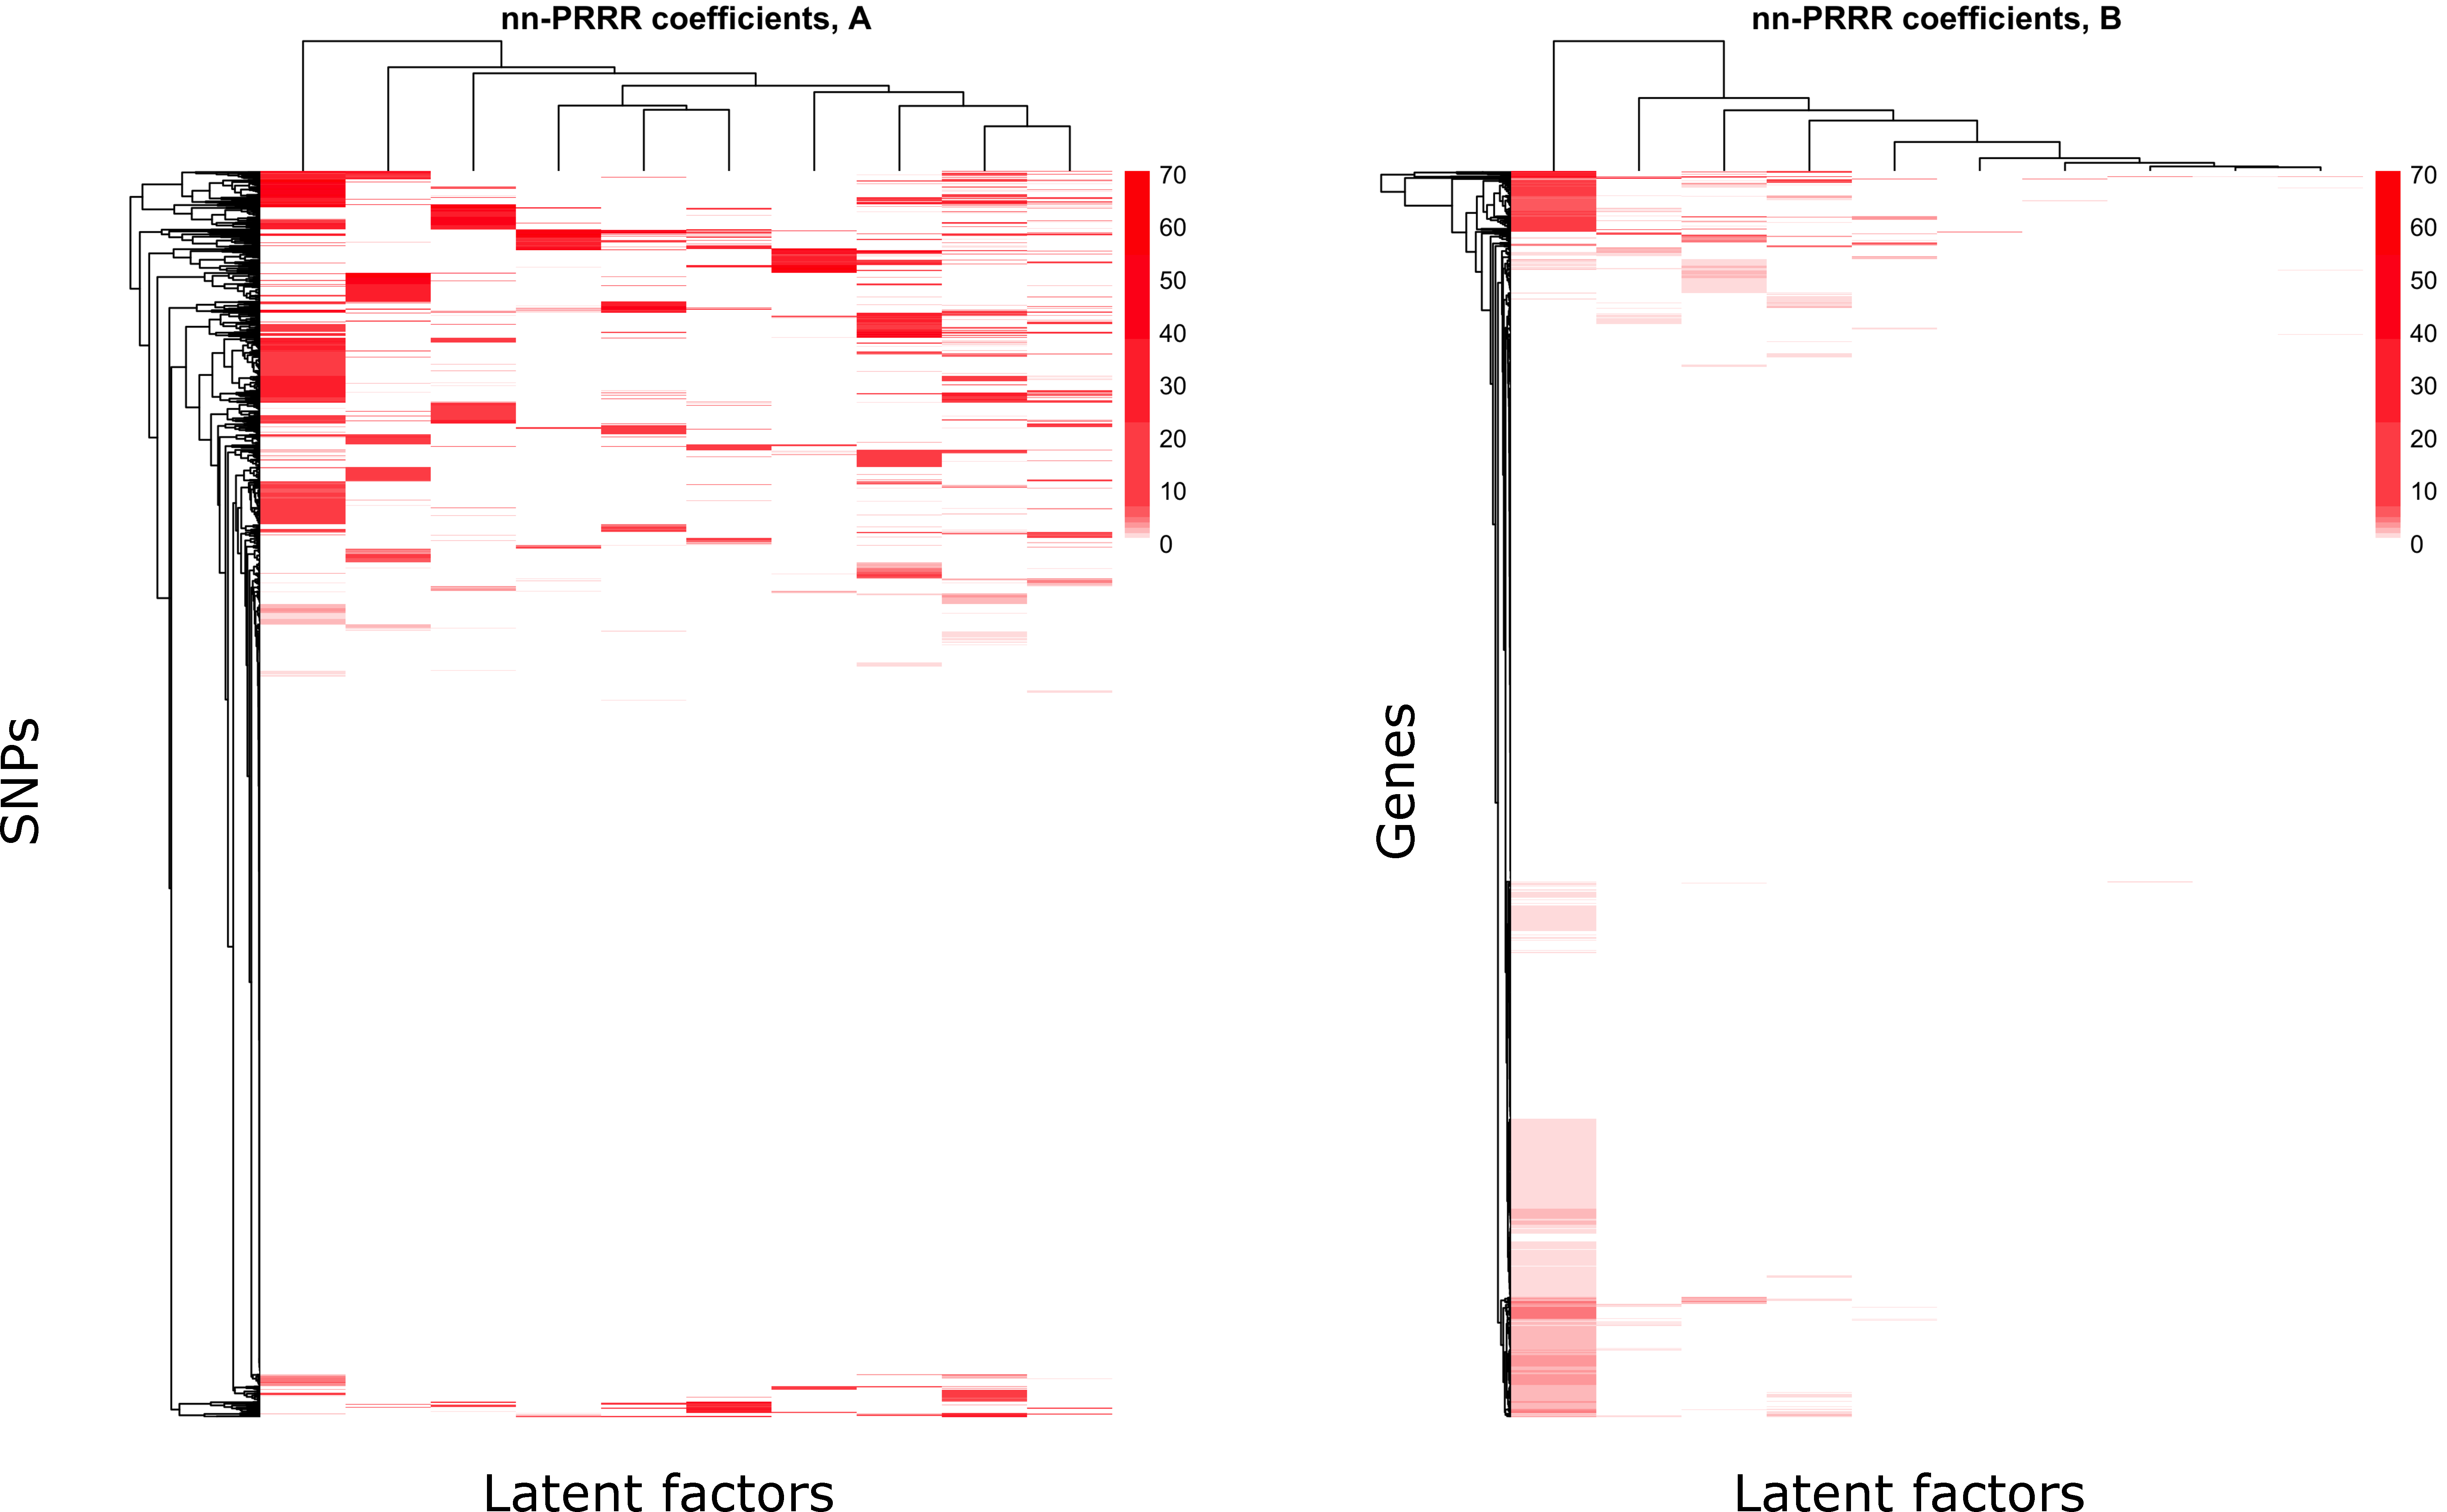
\includegraphics[width=0.9\textwidth]{figures/supplementary_figure5.pdf}
\caption{\csentence{nn-PRRR coefficients for GTEx eQTL mapping.} Left: $\mathbf{U}$ matrix showing SNPs on the rows and latent factors on the columns. Right: $\mathbf{V}$ matrix showing genes on the rows and latent factors on the columns.}
\label{fig:heatmap_fig_prrr}
\end{figure}


% \end{backmatter}
\end{document}
